\documentclass{beamer}
\usepackage[utf8]{inputenc}
\usepackage{color}
\usepackage{fancybox}
\usepackage{graphicx}
\usepackage{booktabs}
\usepackage{amsmath}
\usepackage{amssymb}
\usepackage{xcolor}
\usepackage{pgfplots}
\usepackage{ulem}
\usepackage{listings}
\usepackage{beamerthemesplit}
\usepackage{beamerthemeHeidelberg}
\definecolor{RoyalBlue}{cmyk}{1, 0.50, 0, 0}
\definecolor{geen}{cmyk}{1, 0, .9, 0}
\newtheorem{bla}{Definition}[section]
\lstset{
	language=Python,
	keywordstyle=\color{RoyalBlue},
	basicstyle=\scriptsize\ttfamily,
	breaklines=true,
	gobble=24
}

\usetheme{Heidelberg}
\definecolor{unirot}{rgb}{0.5976525,0,0}
\usecolortheme[named=unirot]{structure}

\title[Vorkurs: AlDa]{Vorkursvortrag: Algorithmen und Datenstrukturen}
\subtitle{Vorkurs WiSe 2023/24}
\author[Raeesa Yousaf]{Raeesa Yousaf, raeeesa@mathphys.info}
\date{\today}
\institute[Uni HD]{
	Ruprecht-Karls-Universität Heidelberg \\
	}

\AtBeginSection[]{
	\begin{frame}<beamer>
		\frametitle{Inhalt}
		\tableofcontents[currentsection, hideallsubsections]
	\end{frame}
}


\begin{document}
	\frame[plain]{\titlepage}
	\frame{\frametitle{Inhalt}\tableofcontents[hideallsubsections]}
	\section[Suchalgorithmen]{Algorithmen: Suchen}
	\frame{
		\frametitle{Was ist ein Algorithmus?}
		"Algorithmen" sind überall! \pause\\
		\begin{itemize}
			\item Firmen nutzen Algorithmen für "streamlining of workflow"
			\item Soziale Netzwerke nutzen Algorithmen für content recommendations
			\item Etc... \pause\\
		\end{itemize}
		Was heißt dieses Wort denn überhaupt?
	}
	\frame{
		\frametitle{Definition Algorithmus}
		\begin{block}{\textbf{Definition 1.1:} Algorithmus}
			Ein Algorithmus ist eine Liste von \textcolor{RoyalBlue}{endlich vielen}, \textcolor{geen}{elementaren} Schritten, um ein Problem zu lösen.
		\end{block}
		Beispiele: Kuchen backen, IKEA-Möbel zusammenbauen, Quests in Videospielen...\\ \pause
		Für Unsere Zwecke: Suchen, Sortieren
	}
	\frame{
		\frametitle{Suchen}
		\begin{block}{\textbf{Definition 1.2:} Suchen}
			Einen \textcolor{RoyalBlue}{Suchbereich} durchlaufen und Elemente mit \textcolor{geen}{gewissen Charakteristiken} finden.
		\end{block}
		Charakteristiken: ist gleich, größer als, Hamming-Distanz kleiner als 2, ...\\\pause
		Suchverfahren:
		\begin{itemize}
			\item Linear
			\item Binär
		\end{itemize}
		(für unsere Zwecke: Liste mit Zufallszahlen; suche ein bestimmtes Element)
	}
	\begin{frame}[fragile]
		\frametitle{Lineare Suche}
		Laufe die Liste von Anfang an durch und vergleiche alle Elemente mit dem, welches wir suchen\\\pause
		\begin{lstlisting}
			for i in range(10):
				if list[i]==gesucht:
					return list[i]
			return NULL
		\end{lstlisting}
		Ist die einzige Option, wenn die Liste nicht sortiert ist.
	\end{frame}
	\begin{frame}[fragile]
		\frametitle{Binäre Suche}
		Funktioniert nur, wenn die Liste sortiert ist!\\
		\begin{enumerate}
			\item Finde die Mitte der Liste
			\item Vergleiche den Wert mit dem, der gesucht wird
			\item Wenn der gesuchte Wert größer ist als die Mitte, wiederhole den Prozess mit der oberen Hälfte; analog mit der unteren Hälfte\\\pause
		\end{enumerate}
		\begin{lstlisting}
			min = 0
			max = x-1
			while min <= max:
				i=math.ceil((max+min)/2.0)
				if gesucht > list[i]:
					min = i+1
				elif gesucht < list[i]:
					max = i-1
				else:
					return list[i]
			return NULL
		\end{lstlisting}
	\end{frame}
	\frame{
		\frametitle{Frage:}
		Intuitiv sieht man ja, dass die zweite Art zu suchen schneller ist...\pause\\
		... aber wie kann man dies wissenschaftlich ausdrücken?
	}
	\section[Landau]{Landau-Notation}
	\frame{
		\frametitle{Landau-Notation}
		\begin{itemize}
			\item Auch bekannt als: Landau-Symbole, big O notation
			\item Erfunden von Paul Bachmann und Edmund Landau
			\item Beschreiben das asymptotische Verhalten von Funktionen und Folgen
			\item Beantworten die Frage: “Wenn meine Liste x-mal so groß wäre, wie viel mehr Aufwand/Speicher/Zeit brauch ich, um das Problem zu lösen?”
			\item Fünf Symbole: \(o, \mathcal{O}, \Theta, \Omega, \omega\) (aber fürs Erste ist nur \(\mathcal{O}\) wichtig)
		\end{itemize}
	}
	\frame{
		\frametitle{Das Landau-O}
		\begin{itemize}
			\item Notation \(g(x)\in \mathcal{O}(f(x))\)
			\item Bedeutet: g(x) ist ungefähr gleich komplex wie f(x) (oder weniger)
			\item Beispiel: “Suche mir im Telefonbuch den allerersten Namen raus” = \(\mathcal{O}(1)\)
			\item Beispiel: “Drucke bitte n Seiten aus” = \(\mathcal{O}(n)\)
			\item Wichtig: Doppelseitig oder nicht ist irrelevant!
		\end{itemize}
	}
	\frame{
		\frametitle{Komplexität: Suchen}
		Lineares Suchen:\\
		Man muss jedes Element überprüfen, bis man das Richtige findet; Bei doppelt so langer Liste muss man doppelt so lange suchen \(\Rightarrow \mathcal{O}(n)\)  \\[2\baselineskip]
		Binäres Suchen:\\
		Nach jedem Schritt wird der Suchbereich halbiert; Bei doppelt so langer Liste nur einen Schritt mehr \(\Rightarrow \mathcal{O}(\log n)\)
	}
	\frame{
		\frametitle{Komplexität: Suchen}
		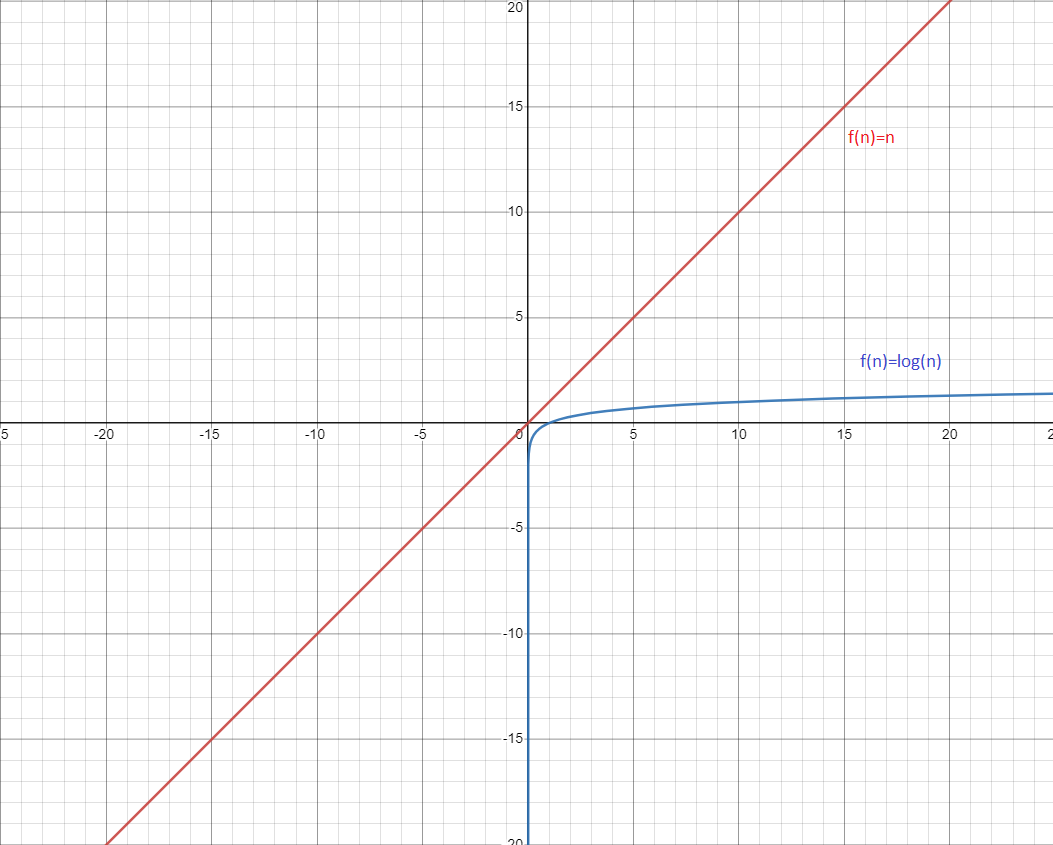
\includegraphics[scale=.3]{komplexitaet}
	}
	\frame{
		\frametitle{Komplexität}
		Wichtig: Nur weil ein Algorithmus ein “besseres \(\mathcal{O}\)” hat, heißt es (im echten Leben) nicht immer, dass der Algorithmus besser/schneller/etc... ist!
	}
	\section[Sortieralgorithmus]{Algorithmen: Sortieren}
	\frame{
		\begin{block}{\textbf{Definition 1.3:} Sortieren}
			Elemente im Sortierbereich in eine \textcolor{RoyalBlue}{von einer Charakteristik abhängigen Reihenfolge} bringen.
		\end{block}
		\pause
		\begin{itemize}
			\item Insertion Sort
			\item Selection Sort
			\item Bubblesort
			\item Mergesort
			\item Quicksort
			\item Miscsort
		\end{itemize}
	}
	\begin{frame}[fragile]
		\frametitle{Insertion Sort}
		\begin{itemize}
			\item Fange am Anfang an
			\item Sortiere bei jedem Schritt das “linkeste” Element des noch unsortierten Teils der Liste in den sortierten Teil der Liste ein\pause
		\end{itemize}
		\begin{lstlisting}
			for i in range(1, len(arr)): 
    				key = arr[i] 
    				j = i-1
    				while j >=0 and key < arr[j] : 
    					arr[j+1] = arr[j] 
    					j -= 1
    				arr[j+1] = key 
		\end{lstlisting}\pause
		Durchschnittliche Komplexität: \(\mathcal{O}(n^2)\)
	\end{frame}
	\begin{frame}[fragile]
		\frametitle{Selection Sort}
		\begin{itemize}
			\item Fange am Anfang an
			\item Suche bei Schritt n das n-kleinste Element in der unsortierten Liste und tausche dies mit dem Element auf Platz n\pause
		\end{itemize}
		\begin{lstlisting}
			for i in range(len(arr)):
				min_idx = i 
				for j in range(i+1, len(arr)): 
					if arr[min_idx] > arr[j]: 
						min_idx = j 
				arr[i], arr[min_idx] = arr[min_idx], arr[i] 
		\end{lstlisting}\pause
		Durchschnittliche Komplexität: \(\mathcal{O}(n^2)\) (aber idR schlechtere Performance als Insertion Sort!)
	\end{frame}
	\begin{frame}[fragile]
		\frametitle{Bubblesort}
		\begin{itemize}
			\item Fange am Anfang an
			\item Bringe nach jedem Schritt das größte Element so weit nach hinten wie möglich, bis du entweder ein größeres findest oder am Ende angelangst\pause
		\end{itemize}
		\begin{lstlisting}
			n = len(arr) 
			for i in range(n-1): 
				for j in range(0, n-i-1): 
					if arr[j] > arr[j+1] : 
						arr[j], arr[j+1] = arr[j+1], arr[j] 
		\end{lstlisting}\pause
		Durchschnittliche Komplexität: \(\mathcal{O}(n^2)\)
	\end{frame}
	\frame{
		\frametitle{Mergesort}
		\begin{itemize}
			\item Teile die Liste in Einzelteile, bis du nicht mehr kannst
			\item Sortiere die Elemente beim Zusammenfügen wieder\pause
		\end{itemize}
		\texttt{ERROR: CODE ZU LANG FÜR PRÄSENTATION}\\\pause
		Durchschnittliche Komplexität: \(\mathcal{O}(n\log n)\)
	}
	\frame{
		\frametitle{Quicksort}
		\begin{itemize}
			\item Suche dir ein Element als Pivot aus
			\item Füge die restlichen Elemente in eine von zwei Teillisten ein, je nachdem, ob die größer oder kleiner als das Pivot sind
			\item Sortiere die Teillisten\pause
		\end{itemize}
		\texttt{ERROR: CODE ZU LANG FÜR PRÄSENTATION}\\\pause
		Durchschnittliche Komplexität: \(\mathcal{O}(n\log n)\)
	}
	\frame{
		\frametitle{Miscsorts}
		\begin{itemize}
			\item Heapsort \pause
			\item Cocktail shaker sort \pause
			\item Tree sort\pause
			\item Bogosort\pause
			\item QUANTUM Bogosort\pause
			\item Pancake sort\pause
			\item I Can’t Believe It Can sort\pause
			\item ...
		\end{itemize}
	}
	\section[Datenstruktur]{Datenstrukturen}
	\frame{
		\frametitle{Definition Datenstruktur}
		\begin{block}{\textbf{Definition 1.4:} Datenstruktur}
			Eine Datenstruktur ist ein Objekt zur \textcolor{RoyalBlue}{Speicherung und Organisation von Daten}. Dieses Objekt ist durch die enthaltenen Daten, aber vor allem durch \textcolor{geen}{die Operationen auf diesen Daten/dem Objekt} charakterisiert.
		\end{block}\pause
		\begin{itemize}
			\item Array
			\item Vector
			\item (Linked) List
			\item Container\pause
			\begin{itemize}
				\item Stack
				\item Queue
				\item Dictionary
			\end{itemize}
		\end{itemize}
	}
	\frame{
		\frametitle{Array}
		Ein Array ist eine Sammlung einer bestimmten Anzahl von Elementen, die in aufeinanderfolgenden Speicheradressen gespeichert wurden.\\
		\textcolor{geen}{Vorteil}: Schnelle Zugriffe (\(\mathcal{O}(1)\))\\
		\textcolor{red}{Nachteil}: Man kann nicht direkt Elemente hinzufügen
	}
	\frame{
		\frametitle{Vector}
		Auch in aufeinanderfolgenden Adressen gespeichert, aber beliebig erweiterbar\\
		\textcolor{geen}{Vorteil}: genauso schnell wie Array und beliebig erweiterbar\\
		\textcolor{red}{Nachteil}: speicherintensiver als Arrays
	}
	\frame{
		\frametitle{Linked List}
		Liste, wo jedes Element zwei Teile enthält: Einen Wert und einen pointer auf das nächste Element.\\
		\textcolor{geen}{Vorteil}: Wieder flexible Größe, Änderungen zwischen Elementen simpel\\
		\textcolor{red}{Nachteil}: Kein Indexzugriff möglich
	}
	\frame{
		\frametitle{Container}
		Container sind Abstrakte Datentypen, die andere Daten speichern können; Operationen und Semantik werden dazudefiniert
		\begin{itemize}
			\item Stack
			\item Queue
			\item Dictionary
		\end{itemize}
	}
	\frame{
		\frametitle{Container: Stack und Queue}
		Beides sind Container, in denen Elemente “temporär” gespeichert werden, um dann wieder in einer bestimmten Reihenfolge entfernt zu werden;\\[2\baselineskip]
		\begin{tabular}{l r}
			Stack: LIFO & Queue: FIFO\\
			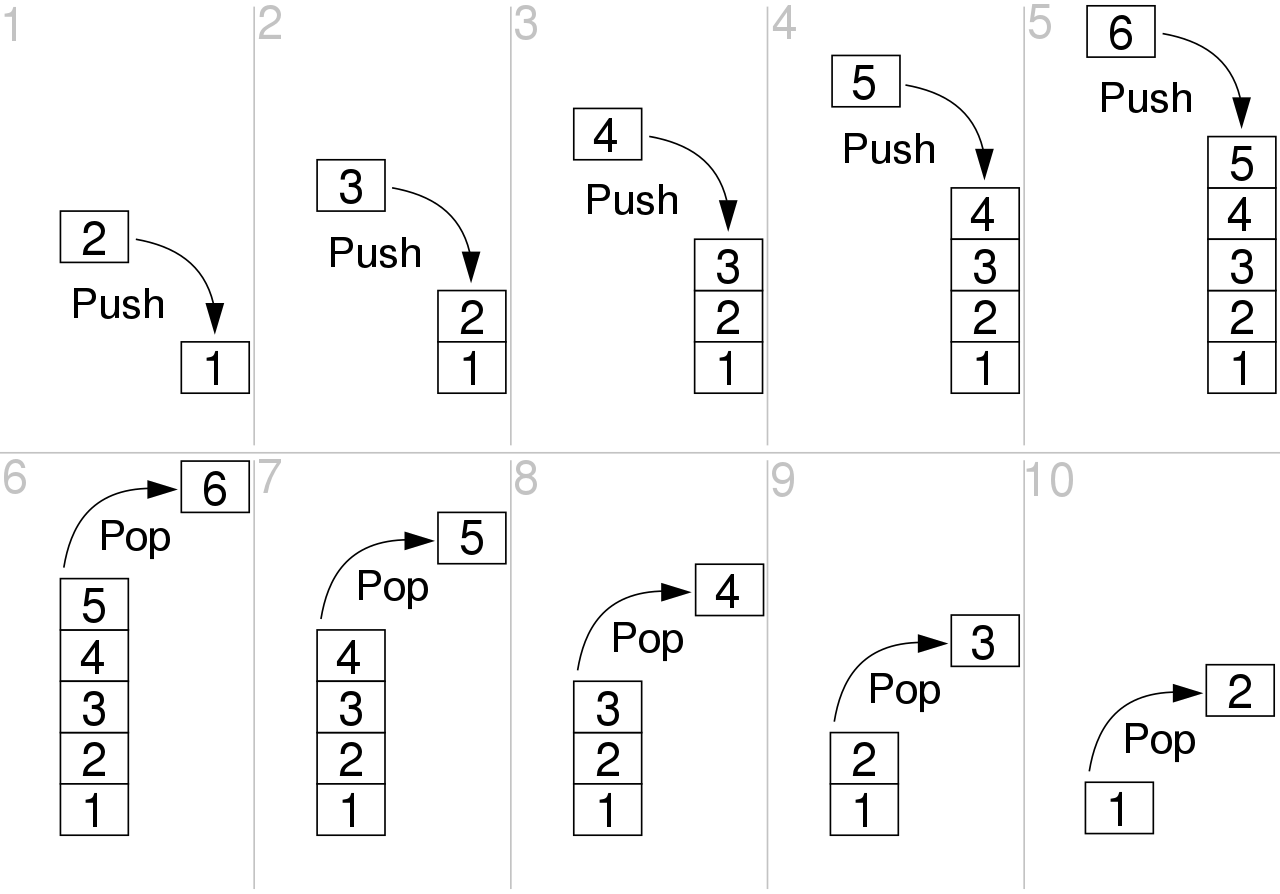
\includegraphics[scale=.1]{Lifo_stack} & 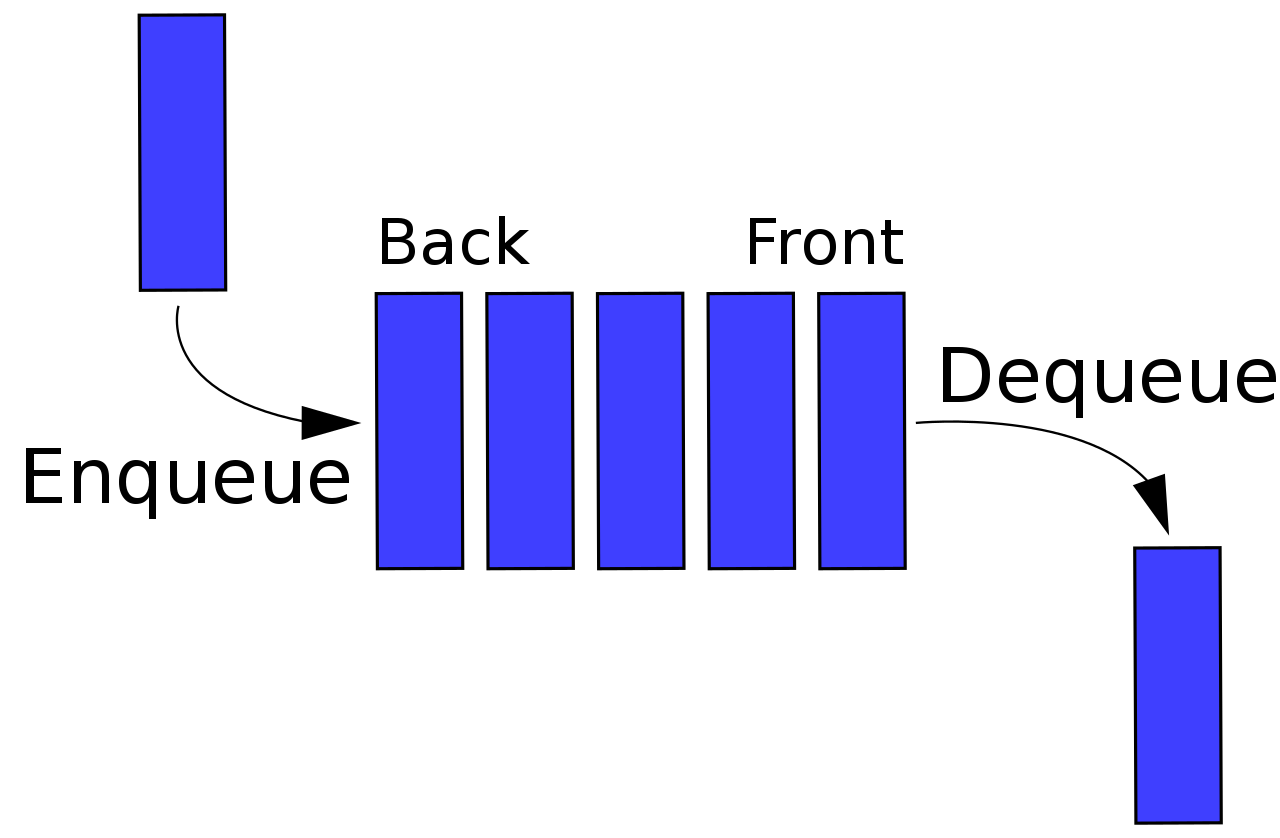
\includegraphics[scale=.1]{Data_Queue}\\
		\end{tabular}
	}
	\frame{
		\frametitle{Container: Dictionary}
		Ein Dictionary speichert Wertepaare; Ein Wertepaar besteht aus “Key” und “Value”\\
		Wird öfter für Lookups benutzt\\
	}
	\section[Fazit]{Fazit}
	\frame{
		\begin{itemize}
			\item Ihr habt die \textit{Absoluten Basics} der Informatik kennengelernt\\\pause
			\item Turingmaschinen, Programmierparadigmen, Klassen/Vererbung, Betriebssysteme, Internet, Datenbanken Und Und Und!!!!!\\\pause
			\item Informatik ist ein vielseitiges und interessantes Gebiet
		\end{itemize}
	}

\end{document}